% The Computational Lab: a scientist drives staged workflows (dev/) that change
% the code under study (app/) and record every step (experiments/).
% Build: latexmk -pdf schematic.tex
\documentclass[tikz, border=4pt]{standalone}
\usetikzlibrary{arrows.meta, positioning, fit, backgrounds}

\tikzset{
  teammate/.pic={
    \fill[#1] (0,0) circle (3.2pt);
    \draw[#1, line width=2.4pt, line cap=round]
      (-4.6pt,-11pt) to[out=90,in=205] (0,-4.6pt) to[out=-25,in=90] (4.6pt,-11pt);
  },
}

\begin{document}
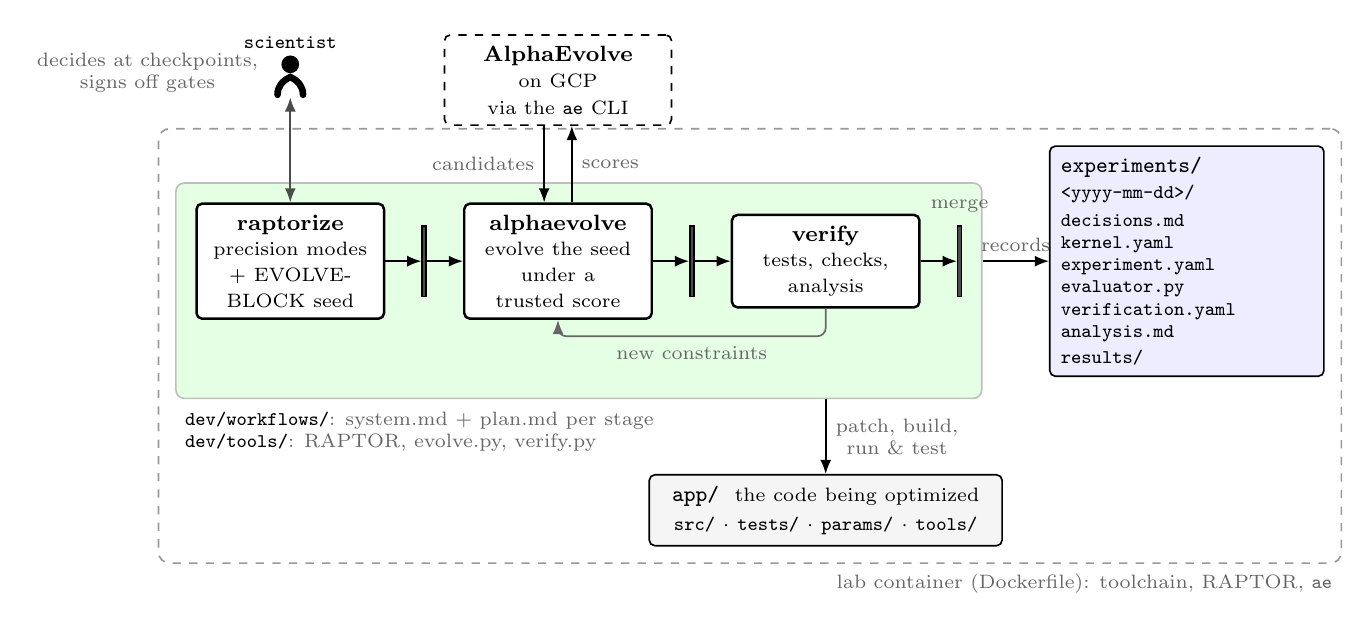
\begin{tikzpicture}[
    font=\footnotesize,
    >={Latex[length=1.8mm, width=1.4mm]},
    every path/.style={line width=0.6pt},
    box/.style={draw, rounded corners=2pt, align=center, inner sep=4pt, fill=white},
    stage/.style={box, line width=0.9pt, text width=2.1cm, minimum height=1.1cm},
    gate/.style={draw, fill=black!70, minimum width=1.4pt, minimum height=0.9cm, inner sep=0pt},
    lbl/.style={font=\scriptsize, text=black!60, align=center},
  ]

  % Stages and the gates between them
  \node[stage] (rap) at (0,0) {\textbf{raptorize}\\[1pt]{\scriptsize precision modes\\+ EVOLVE-BLOCK seed}};
  \node[stage] (ae)  at (3.4,0) {\textbf{alphaevolve}\\[1pt]{\scriptsize evolve the seed\\under a trusted score}};
  \node[stage] (ver) at (6.8,0) {\textbf{verify}\\[1pt]{\scriptsize tests, checks,\\analysis}};
  \node[gate] (g1) at (1.7,0) {};
  \node[gate] (g2) at (5.1,0) {};
  \node[gate] (g3) at (8.5,0) {};
  \draw[->] (rap) -- (g1); \draw[->] (g1) -- (ae);
  \draw[->] (ae) -- (g2);  \draw[->] (g2) -- (ver);
  \draw[->] (ver) -- (g3);
  \node[lbl, above=1pt of g3] {merge};
  \draw[->, rounded corners=3pt, black!60] (ver.south) -- ++(0,-0.35) -| node[lbl, pos=0.25, below] {new constraints} (ae.south);

  % dev/: the agentic layer
  \coordinate (devlow) at ([yshift=-0.75cm]ae.south);
  \begin{scope}[on background layer]
    \node[draw=black!25, rounded corners=3pt, fill=green!10, inner sep=7pt,
          fit=(rap) (ver) (g3) (devlow)] (dev) {};
  \end{scope}
  \node[lbl, anchor=north west, align=left] (devlbl) at ([yshift=-1pt]dev.south west)
    {{\ttfamily\color{black}dev/workflows/}: system.md + plan.md per stage\\
     {\ttfamily\color{black}dev/tools/}: RAPTOR, evolve.py, verify.py};

  % Scientist
  \coordinate (sci) at (0,2.5);
  \path (sci) pic{teammate={black}};
  \node[above=2pt of sci, font=\ttfamily\scriptsize] {scientist};
  \node[lbl, left=8pt of sci, yshift=-3pt] {decides at checkpoints,\\signs off gates};
  \draw[<->, black!70] ([yshift=-0.42cm]sci) -- (rap.north);

  % app/: the code being optimized
  \coordinate (apptop) at ([yshift=-0.95cm]dev.south);
  \node[box, fill=black!4, text width=4.2cm, anchor=north] (app) at (apptop -| ver)
    {\textbf{\ttfamily app/}\ \ {\scriptsize the code being optimized}\\[1pt]
     {\ttfamily\scriptsize src/ $\cdot$ tests/ $\cdot$ params/ $\cdot$ tools/}};
  \draw[->] (dev.south -| app.north) -- node[lbl, right] {patch, build,\\run \& test} (app.north);

  % experiments/: the provenance record
  \node[box, fill=blue!7, text width=3.2cm, align=left, right=1.1cm of g3, anchor=west] (exp)
    {\textbf{\ttfamily experiments/}\\{\ttfamily\scriptsize <yyyy-mm-dd>/}\\[2pt]
     {\ttfamily\scriptsize decisions.md\\kernel.yaml\\experiment.yaml\\evaluator.py\\verification.yaml\\analysis.md\\results/}};
  \draw[->] (dev.east |- exp.west) -- node[lbl, above] {records} (exp.west);

  % AlphaEvolve service
  \node[box, dashed, text width=2.6cm] (gcp) at (3.4,2.3)
    {\textbf{AlphaEvolve} {\scriptsize on GCP}\\{\scriptsize via the \ttfamily ae\normalfont\ CLI}};
  \coordinate (down) at ([xshift=-5pt]gcp.south);
  \coordinate (up) at ([xshift=5pt]gcp.south);
  \draw[->] (down) -- node[lbl, left] {candidates} (down |- ae.north);
  \draw[<-] (up) -- node[lbl, right] {scores} (up |- ae.north);

  % Container boundary
  \begin{scope}[on background layer]
    \node[draw=black!40, dashed, rounded corners=4pt, inner sep=6pt,
          fit=(dev) (app) (exp) (devlbl)] (box) {};
  \end{scope}
  \node[lbl, anchor=north east] at (box.south east) {lab container (Dockerfile): toolchain, RAPTOR, \ttfamily ae};
\end{tikzpicture}
\end{document}
